\def\ReportNumber{1}
\def\ReportName{Cable selection and model setup}
\documentclass[11pt,a4paper]{article}
\usepackage[T1]{fontenc}
\usepackage[utf8]{inputenc}
\usepackage{newtxtext,newtxmath,microtype}
\usepackage[margin=21mm,headheight=14pt]{geometry}
\usepackage{booktabs,tabularx,array,amsmath,graphicx,float,caption}
\usepackage{xcolor,fancyhdr,lastpage,listings}
\usepackage[hidelinks]{hyperref}
\definecolor{accent}{HTML}{254C58}
% Original question wording: NMES Assignment 2026, Sections 1--3.
% Line-wrap hyphenation is removed; mathematical notation is typeset in LaTeX.
\usepackage{tcolorbox}
\newcommand{\assignmentquestion}[1]{%
  \begin{tcolorbox}[colback=accent!4,colframe=accent!65,
    boxrule=0.4pt,leftrule=2pt,arc=0pt,boxsep=0pt,
    left=7pt,right=7pt,top=5pt,bottom=5pt,
    before skip=0pt,after skip=8pt,fontupper=\small]
  \textbf{Assignment question.} #1
  \end{tcolorbox}%
}
\newcommand{\questionfiles}[1]{%
  \par\smallskip{\footnotesize\color{accent}
  \textbf{Files / results (relative to Source-code).} #1\par}\medskip
}
\newcommand{\QuestionOneOne}{%
Describe your cable: construction, dimensions, materials, rated voltage, rated
current (ampacity) and the laying conditions for which that rating is given
(burial depth, soil thermal resistivity, ambient temperature, arrangement).
Give a table of electromagnetic and thermal properties with a source for each value.}
\newcommand{\QuestionOneTwo}{%
Choose the environment consistently with the datasheet rating conditions,
and justify its properties.}
\newcommand{\QuestionOneThree}{%
State the sheath bonding you assume: single-point bonded (no net sheath current)
or solidly bonded (circulating sheath currents allowed), and how the armour
and pipe are connected. This choice strongly affects the losses in Section 3.}
\newcommand{\QuestionOneFour}{%
State the excitation you impose: phase-to-ground voltage and phase current,
as peak phasors, with the phase sequence (see the conventions in Appendix A).}
\newcommand{\QuestionTwoOne}{%
Define your computational domain, the equations solved and the boundary
conditions. Where do you truncate the domain, and why? Discuss the role of
the grounded screens: which regions actually influence the field in the insulation?}
\newcommand{\QuestionTwoTwo}{%
Can you simplify the geometry of your cable without degrading the precision
(e.g. disregard details in the geometrical description)? Quantify the effect
of each simplification.}
\newcommand{\QuestionTwoThree}{%
How do the results vary with the mesh refinement? Plot the maximum field in
the insulation and the capacitance versus the number of degrees of freedom,
and identify where local refinement is needed.}
\newcommand{\QuestionTwoFour}{%
Define the admissible field strength at the conductor screen and at the core
screen from the datasheet (or, if absent, from a cited reference).
Is the healthy cable within these limits?}
\newcommand{\QuestionTwoFive}{%
Add a defect to the insulation of your cable. State its nature (e.g. gas void,
water tree, protrusion of the semiconducting screen), its properties, size and
position, and discuss what a defect in a 2D cross-section represents in 3D.
Compare the field with and without defect along a radial cut.
Does the cable withstand the defect?}
\newcommand{\QuestionTwoSix}{%
Compute the resistive and displacement current densities in the cable.
Is current conservation satisfied? Which current dominates in each material, and why?}
\newcommand{\QuestionTwoSeven}{%
Compute the per-unit-length capacitance (\(\mu\mathrm{F/km}\)) and compare with
the analytical value (13) and with the datasheet. State the assumptions of the
analytical formula (in particular, how the semiconducting layers are treated).
Does the capacitance vary with frequency? Why (not)?}
\newcommand{\QuestionTwoEight}{%
Propose an improvement of the cable design with respect to the electric stress,
and support it quantitatively.}
\newcommand{\QuestionThreeOne}{%
Define your computational domain, the equations solved and the boundary conditions.
Where do you truncate the domain, and why? How do you impose the currents in the phase conductors?}
\newcommand{\QuestionThreeTwo}{%
\textbf{Conductor model.} Compare the skin depth in the conductor with its radius.
Model the phase conductors (a) as stranded conductors (imposed uniform current density)
and (b) as massive conductors (imposed net current, eddy currents allowed).
Which assumption is more realistic for your cable, and how does it affect the results?}
\newcommand{\QuestionThreeThree}{%
\textbf{Bonding.} Implement the bonding assumed in Q1.3 with global quantities
(net current and voltage per unit length in the sheaths, armour and pipe).
Explain why using only \(\mathbf j=-\mathrm i\omega\sigma\mathbf a\)
in these regions does not correspond to a well-defined bonding condition.}
\newcommand{\QuestionThreeFour}{%
Can you simplify the geometry without degrading the precision?
Are the simplifications of Section 2 still valid here?}
\newcommand{\QuestionThreeFive}{%
Check the mesh quality and refine where needed (element size compared with the
skin depth in each conducting region). How do losses, resistance and inductance
vary with the mesh refinement?}
\newcommand{\QuestionThreeSix}{%
Get the magnetic flux density (or induction) in and around your cable.}
\newcommand{\QuestionThreeSeven}{%
Get the current density in the conducting parts of your cable.}
\newcommand{\QuestionThreeEight}{%
Get the time-averaged Joule losses (kW/km) in each conducting part
(conductors, sheaths, armour, pipe, environment).}
\newcommand{\QuestionThreeNine}{%
Get the per-unit-length AC resistance (\(\Omega/\mathrm{km}\)), defined from
the total losses. Compare it with the DC resistance and with the datasheet.
Separate the contributions of skin/proximity effect and of sheath/armour losses.}
\newcommand{\QuestionThreeTen}{%
Get the per-unit-length inductance (mH/km). How do you define it for a
three-phase system? Does it vary with frequency? Compare with the datasheet.}
\newcommand{\QuestionThreeEleven}{%
Propose a design change that reduces the losses, and support it quantitatively.}

\pagestyle{fancy}\fancyhf{}
\fancyhead[L]{\small FE for Electromagnetic Fields -- Kutikuppala, Lefebure, Miseur}
\fancyhead[R]{\small NKT 33 kV, 185 + 50 mm\textsuperscript{2}}
\fancyfoot[L]{\small Section \ReportNumber\ -- \ReportName}
\fancyfoot[R]{\small\thepage\,/\,\pageref{LastPage}}
\renewcommand{\headrulewidth}{0.3pt}
\setlength{\parindent}{0pt}\setlength{\parskip}{5pt}
\setlength{\emergencystretch}{2em}
\setlength{\tabcolsep}{5pt}\renewcommand{\arraystretch}{1.13}
\captionsetup{font=small,labelfont=bf,skip=5pt}
\newcolumntype{Y}{>{\raggedright\arraybackslash}X}
\newcommand{\file}[1]{\href{../Source-code/#1}{\nolinkurl{#1}}}
\newcommand{\setupfile}[1]{\file{Cable-selection-and-model-setup/#1}}
\newcommand{\efile}{\file{Electrodynamic-analysis/cable.pro}}
\newcommand{\mfile}{\file{Magnetothermal-analysis/cable.pro}}
\newcommand{\runall}{\href{../run_all.sh}{\nolinkurl{run_all.sh}}}
\newcommand{\runE}{\texttt{getdp cable.pro -msh}\ \path{../Cable-selection-and-model-setup/cable.msh}\ \texttt{-solve Electrodynamics}}
\newcommand{\codeguide}[3]{\par\smallskip
 {\small\bfseries\color{accent}Code guide}\par\nobreak
 \begingroup\small\setlength{\tabcolsep}{0pt}
 \begin{tabularx}{\linewidth}{@{}p{14mm}Y@{}}
 \textbf{Files} & #1\\[2pt]
 \textbf{Run} & #2\\[2pt]
 \textbf{Check} & #3
 \end{tabularx}\par\endgroup\medskip}
\newcommand{\pending}{\textbf{Status: implementation still required.} }
\newcommand{\refurl}[2]{\href{#1}{#2}}
\lstset{basicstyle=\small\ttfamily,columns=fullflexible,keepspaces=true,
 showstringspaces=false,breaklines=true,upquote=true,
 backgroundcolor=\color{accent!4},frame=none,
 xleftmargin=5pt,xrightmargin=5pt,aboveskip=5pt,belowskip=5pt}
\hypersetup{pdftitle={Section \ReportNumber: \ReportName},
  pdfauthor={Kutikuppala Jaswanth, Lefebure Tiebert, Miseur Torre}}

\graphicspath{{../../Slides/figures/}}
% Generated by Reports/collect_values.py. Do not edit.
\newcommand{\AmpLin}{386}
\newcommand{\Ampflat}{343}
\newcommand{\Ampflatsev}{352}
\newcommand{\Ampflatsevsp}{374}
\newcommand{\Ampflatsp}{351}
\newcommand{\Amptrefoil}{345}
\newcommand{\Amptrefoilsp}{350}
\newcommand{\AnaC}{0.197031}
\newcommand{\AnaCbare}{0.1834}
\newcommand{\AnaCthick}{0.181271}
\newcommand{\AnaDeltaAl}{11.96}
\newcommand{\AnaDeltaCu}{9.35}
\newcommand{\AnaDrop}{7}
\newcommand{\AnaEb}{5.14}
\newcommand{\AnaEi}{4.894}
\newcommand{\AnaEirms}{3.46}
\newcommand{\AnaEithick}{4.502}
\newcommand{\AnaEorms}{1.71}
\newcommand{\AnaEvoid}{6.20}
\newcommand{\AnaEzero}{4.34}
\newcommand{\AnaIch}{1.179}
\newcommand{\AnaJc}{\ensuremath{4.89\cdot10^{-12}}}
\newcommand{\AnaJd}{0.0340}
\newcommand{\AnaLgap}{0.4043}
\newcommand{\AnaLtouch}{0.4019}
\newcommand{\AnaRatio}{\ensuremath{1.44\cdot10^{-10}}}
\newcommand{\AnaWd}{0.022}
\newcommand{\AnaWdShare}{0.09}
\newcommand{\Bmax}{15.6}
\newcommand{\Bsingle}{13.4}
\newcommand{\Cdefect}{0.197000}
\newcommand{\Cdefectfine}{0.196999}
\newcommand{\Cffive}{0.197032}
\newcommand{\Cfhund}{0.197032}
\newcommand{\Cfthou}{0.197032}
\newcommand{\Cgap}{0.197032}
\newcommand{\Cgapcoarse}{0.197044}
\newcommand{\Cgapfine}{0.197031}
\newcommand{\CondShare}{94}
\newcommand{\ConvRate}{0.22}
\newcommand{\Cqdefect}{0.196937}
\newcommand{\Cqdefectfine}{0.196935}
\newcommand{\Cqffive}{0.197032}
\newcommand{\Cqfhund}{0.197032}
\newcommand{\Cqfthou}{0.197032}
\newcommand{\Cqgap}{0.197032}
\newcommand{\Cqgapcoarse}{0.197044}
\newcommand{\Cqgapfine}{0.197031}
\newcommand{\Cqthick}{0.181272}
\newcommand{\Cqtouching}{0.197032}
\newcommand{\Cthick}{0.181272}
\newcommand{\Ctouching}{0.197032}
\newcommand{\Dofsdefect}{65\,900}
\newcommand{\Dofsdefectfine}{265\,156}
\newcommand{\Dofsffive}{64\,884}
\newcommand{\Dofsfhund}{64\,884}
\newcommand{\Dofsfthou}{64\,884}
\newcommand{\Dofsgap}{64\,884}
\newcommand{\Dofsgapcoarse}{16\,100}
\newcommand{\Dofsgapfine}{261\,058}
\newcommand{\Dofsthick}{76\,210}
\newcommand{\Dofstouching}{64\,880}
\newcommand{\EddyFE}{0.9}
\newcommand{\Edefect}{6.29}
\newcommand{\Edefectfine}{6.30}
\newcommand{\Effive}{4.873}
\newcommand{\Efhund}{4.873}
\newcommand{\Efthou}{4.873}
\newcommand{\Egap}{4.873}
\newcommand{\Egapcoarse}{4.846}
\newcommand{\Egapfine}{4.885}
\newcommand{\Ethick}{4.474}
\newcommand{\Etouching}{4.872}
\newcommand{\Hrad}{5.2}
\newcommand{\Ibalance}{\ensuremath{4\cdot10^{-14}}}
\newcommand{\IchFE}{1.179}
\newcommand{\IecAmp}{351}
\newcommand{\IecIs}{56.8}
\newcommand{\IecLam}{5.52}
\newcommand{\IecLamHot}{3.6}
\newcommand{\IecPc}{60.55}
\newcommand{\IecPcHot}{76.8}
\newcommand{\IecPs}{3.34}
\newcommand{\IecPsHot}{2.76}
\newcommand{\IecPt}{63.89}
\newcommand{\IecRac}{0.1739}
\newcommand{\IecRacHot}{0.2164}
\newcommand{\IecRcond}{0.16475}
\newcommand{\IecRcondHot}{0.2089}
\newcommand{\IecRs}{0.3448}
\newcommand{\IecTfour}{2.236}
\newcommand{\IecTheta}{89.2}
\newcommand{\IecThetaS}{77}
\newcommand{\IecTone}{0.476}
\newcommand{\IecTthree}{0.104}
\newcommand{\IecU}{46.5}
\newcommand{\IecUs}{19.9}
\newcommand{\IecX}{0.0568}
\newcommand{\IecYp}{0.15}
\newcommand{\IecYs}{0.31}
\newcommand{\IecYsp}{0.46}
\newcommand{\Ioneflat}{341}
\newcommand{\Ioneflatsev}{353}
\newcommand{\Ioneflatsevsp}{381}
\newcommand{\Ioneflatsp}{351}
\newcommand{\Ionetrefoil}{344}
\newcommand{\Ionetrefoilsp}{350}
\newcommand{\IratioFE}{\ensuremath{1.44\cdot10^{-10}}}
\newcommand{\IsPeak}{79}
\newcommand{\IsSum}{0.15}
\newcommand{\Isbase}{55.5}
\newcommand{\Isbox}{55.9}
\newcommand{\Iscoarse}{54.9}
\newcommand{\Isfdc}{0.0}
\newcommand{\Isffive}{5.7}
\newcommand{\Isfhund}{267.6}
\newcommand{\Isfine}{55.8}
\newcommand{\Isflat}{60.9}
\newcommand{\IsflatIone}{60.0}
\newcommand{\Isflatsev}{95.4}
\newcommand{\IsflatsevIone}{95.9}
\newcommand{\Isflatsevsp}{0.0}
\newcommand{\IsflatsevspIone}{0.0}
\newcommand{\Isflatsp}{0.0}
\newcommand{\IsflatspIone}{0.0}
\newcommand{\Islin}{55.5}
\newcommand{\Isliniso}{55.5}
\newcommand{\Isnl}{45.4}
\newcommand{\Isnlcoarse}{45.0}
\newcommand{\Isnldomforty}{45.4}
\newcommand{\Isnldomten}{45.4}
\newcommand{\Isnlfine}{45.5}
\newcommand{\Isnlhfive}{45.2}
\newcommand{\Isnlhtwenty}{45.5}
\newcommand{\Isnliso}{45.6}
\newcommand{\Issingle}{0.0}
\newcommand{\Isstranded}{55.6}
\newcommand{\Isstrandedfhund}{268.1}
\newcommand{\Istouching}{54.9}
\newcommand{\Istrefoil}{45.4}
\newcommand{\IstrefoilIone}{45.0}
\newcommand{\Istrefoilsp}{0.0}
\newcommand{\IstrefoilspIone}{0.0}
\newcommand{\Javg}{2.88}
\newcommand{\JcFE}{\ensuremath{4.87\cdot10^{-12}}}
\newcommand{\JdFE}{0.0339}
\newcommand{\Jmax}{3.07}
\newcommand{\Jscreen}{1.6}
\newcommand{\LamFE}{6.1}
\newcommand{\Lbase}{0.3943}
\newcommand{\Lbox}{0.3955}
\newcommand{\Lcoarse}{0.3922}
\newcommand{\Lfdc}{0.4010}
\newcommand{\Lffive}{0.4010}
\newcommand{\Lfhund}{0.2616}
\newcommand{\Lfine}{0.3952}
\newcommand{\Lflat}{0.4331}
\newcommand{\LflatIone}{0.4328}
\newcommand{\Lflatsev}{0.5722}
\newcommand{\LflatsevIone}{0.5724}
\newcommand{\Lflatsevsp}{0.6061}
\newcommand{\LflatsevspIone}{0.6061}
\newcommand{\Lflatsp}{0.4437}
\newcommand{\LflatspIone}{0.4437}
\newcommand{\Llin}{0.3943}
\newcommand{\Lliniso}{0.3943}
\newcommand{\Lnl}{0.3965}
\newcommand{\Lnlcoarse}{0.3944}
\newcommand{\Lnldomforty}{0.3965}
\newcommand{\Lnldomten}{0.3965}
\newcommand{\Lnlfine}{0.3975}
\newcommand{\Lnlhfive}{0.3966}
\newcommand{\Lnlhtwenty}{0.3965}
\newcommand{\Lnliso}{0.3965}
\newcommand{\Lsingle}{0.4003}
\newcommand{\Lstranded}{0.3947}
\newcommand{\Lstrandedfhund}{0.2670}
\newcommand{\Lterm}{0.3945}
\newcommand{\Ltouching}{0.3923}
\newcommand{\Ltrefoil}{0.3965}
\newcommand{\LtrefoilIone}{0.3965}
\newcommand{\Ltrefoilsp}{0.4006}
\newcommand{\LtrefoilspIone}{0.4006}
\newcommand{\MDofsbase}{295\,294}
\newcommand{\MDofsbox}{297\,138}
\newcommand{\MDofscoarse}{75\,856}
\newcommand{\MDofsfdc}{295\,294}
\newcommand{\MDofsffive}{295\,294}
\newcommand{\MDofsfhund}{295\,294}
\newcommand{\MDofsfine}{1\,169\,120}
\newcommand{\MDofsflat}{243\,780}
\newcommand{\MDofsflatIone}{243\,780}
\newcommand{\MDofsflatsev}{253\,538}
\newcommand{\MDofsflatsevIone}{253\,538}
\newcommand{\MDofsflatsevsp}{253\,538}
\newcommand{\MDofsflatsevspIone}{253\,538}
\newcommand{\MDofsflatsp}{243\,780}
\newcommand{\MDofsflatspIone}{243\,780}
\newcommand{\MDofslin}{295\,294}
\newcommand{\MDofsliniso}{295\,294}
\newcommand{\MDofsnl}{295\,294}
\newcommand{\MDofsnlcoarse}{75\,856}
\newcommand{\MDofsnldomforty}{295\,294}
\newcommand{\MDofsnldomten}{295\,294}
\newcommand{\MDofsnlfine}{1\,169\,120}
\newcommand{\MDofsnlhfive}{295\,294}
\newcommand{\MDofsnlhtwenty}{295\,294}
\newcommand{\MDofsnliso}{295\,294}
\newcommand{\MDofssingle}{295\,294}
\newcommand{\MDofsstranded}{295\,288}
\newcommand{\MDofsstrandedfhund}{295\,288}
\newcommand{\MDofstouching}{292\,266}
\newcommand{\MDofstrefoil}{295\,294}
\newcommand{\MDofstrefoilIone}{295\,294}
\newcommand{\MDofstrefoilsp}{295\,294}
\newcommand{\MDofstrefoilspIone}{295\,294}
\newcommand{\MeshBadGap}{0}
\newcommand{\MeshBadTouch}{24}
\newcommand{\MeshQminGap}{0.575}
\newcommand{\MeshQminTouch}{0.020}
\newcommand{\MeshTriGap}{297\,943}
\newcommand{\MeshTriTouch}{294\,915}
\newcommand{\MeshXlpeGap}{22\,228}
\newcommand{\MeshXlpeTouch}{22\,222}
\newcommand{\Nitflat}{10}
\newcommand{\NitflatIone}{10}
\newcommand{\Nitflatsev}{9}
\newcommand{\NitflatsevIone}{9}
\newcommand{\Nitflatsevsp}{10}
\newcommand{\NitflatsevspIone}{11}
\newcommand{\Nitflatsp}{10}
\newcommand{\NitflatspIone}{10}
\newcommand{\Nitlin}{1}
\newcommand{\Nitliniso}{1}
\newcommand{\Nitnl}{10}
\newcommand{\Nitnlcoarse}{10}
\newcommand{\Nitnldomforty}{10}
\newcommand{\Nitnldomten}{10}
\newcommand{\Nitnlfine}{10}
\newcommand{\Nitnlhfive}{10}
\newcommand{\Nitnlhtwenty}{10}
\newcommand{\Nitnliso}{10}
\newcommand{\Nittrefoil}{10}
\newcommand{\NittrefoilIone}{10}
\newcommand{\Nittrefoilsp}{10}
\newcommand{\NittrefoilspIone}{10}
\newcommand{\NktL}{0.382}
\newcommand{\PcPhase}{20.18}
\newcommand{\Pcbase}{60.55}
\newcommand{\Pcbox}{60.55}
\newcommand{\Pccoarse}{60.58}
\newcommand{\Pcfdc}{60.28}
\newcommand{\Pcffive}{60.28}
\newcommand{\Pcfhund}{75.76}
\newcommand{\Pcfine}{60.54}
\newcommand{\Pcflat}{77.44}
\newcommand{\PcflatIone}{72.36}
\newcommand{\Pcflatsev}{76.02}
\newcommand{\PcflatsevIone}{77.69}
\newcommand{\Pcflatsevsp}{73.63}
\newcommand{\PcflatsevspIone}{91.14}
\newcommand{\Pcflatsp}{76.37}
\newcommand{\PcflatspIone}{77.04}
\newcommand{\PcircFE}{3.16}
\newcommand{\Pclin}{60.55}
\newcommand{\Pcliniso}{60.55}
\newcommand{\Pcnl}{77.58}
\newcommand{\Pcnlcoarse}{77.38}
\newcommand{\Pcnldomforty}{77.59}
\newcommand{\Pcnldomten}{77.51}
\newcommand{\Pcnlfine}{77.65}
\newcommand{\Pcnlhfive}{77.92}
\newcommand{\Pcnlhtwenty}{77.40}
\newcommand{\Pcnliso}{77.21}
\newcommand{\Pcsingle}{60.55}
\newcommand{\Pcstranded}{60.26}
\newcommand{\Pcstrandedfhund}{60.26}
\newcommand{\Pctouching}{60.55}
\newcommand{\Pctrefoil}{77.58}
\newcommand{\PctrefoilIone}{74.07}
\newcommand{\Pctrefoilsp}{76.94}
\newcommand{\PctrefoilspIone}{76.94}
\newcommand{\PdInception}{16}
\newcommand{\PhaseSym}{0.0004}
\newcommand{\Psbase}{3.68}
\newcommand{\Psbox}{3.74}
\newcommand{\Pscoarse}{3.59}
\newcommand{\Psfdc}{0.00}
\newcommand{\Psffive}{0.04}
\newcommand{\Psfhund}{81.84}
\newcommand{\Psfine}{3.72}
\newcommand{\Psflat}{5.01}
\newcommand{\PsflatIone}{4.81}
\newcommand{\Psflatsev}{12.34}
\newcommand{\PsflatsevIone}{12.51}
\newcommand{\Psflatsevsp}{0.05}
\newcommand{\PsflatsevspIone}{0.05}
\newcommand{\Psflatsp}{0.41}
\newcommand{\PsflatspIone}{0.41}
\newcommand{\Pslin}{3.68}
\newcommand{\Psliniso}{3.68}
\newcommand{\Psnl}{3.03}
\newcommand{\Psnlcoarse}{2.96}
\newcommand{\Psnldomforty}{3.03}
\newcommand{\Psnldomten}{3.03}
\newcommand{\Psnlfine}{3.06}
\newcommand{\Psnlhfive}{3.02}
\newcommand{\Psnlhtwenty}{3.04}
\newcommand{\Psnliso}{3.04}
\newcommand{\Pssingle}{0.52}
\newcommand{\Psstranded}{3.70}
\newcommand{\Psstrandedfhund}{83.03}
\newcommand{\Pstouching}{3.62}
\newcommand{\Pstrefoil}{3.03}
\newcommand{\PstrefoilIone}{2.95}
\newcommand{\Pstrefoilsp}{0.43}
\newcommand{\PstrefoilspIone}{0.43}
\newcommand{\Ptbase}{64.23}
\newcommand{\Ptbox}{64.30}
\newcommand{\Ptcoarse}{64.17}
\newcommand{\Ptfdc}{60.28}
\newcommand{\Ptffive}{60.32}
\newcommand{\Ptfhund}{157.60}
\newcommand{\Ptfine}{64.27}
\newcommand{\Ptflat}{82.45}
\newcommand{\PtflatIone}{77.17}
\newcommand{\Ptflatsev}{88.36}
\newcommand{\PtflatsevIone}{90.20}
\newcommand{\Ptflatsevsp}{73.68}
\newcommand{\PtflatsevspIone}{91.20}
\newcommand{\Ptflatsp}{76.77}
\newcommand{\PtflatspIone}{77.45}
\newcommand{\Ptlin}{64.23}
\newcommand{\Ptliniso}{64.23}
\newcommand{\Ptnl}{80.61}
\newcommand{\Ptnlcoarse}{80.33}
\newcommand{\Ptnldomforty}{80.62}
\newcommand{\Ptnldomten}{80.55}
\newcommand{\Ptnlfine}{80.71}
\newcommand{\Ptnlhfive}{80.94}
\newcommand{\Ptnlhtwenty}{80.43}
\newcommand{\Ptnliso}{80.25}
\newcommand{\Ptsingle}{61.07}
\newcommand{\Ptstranded}{63.96}
\newcommand{\Ptstrandedfhund}{143.29}
\newcommand{\Pttouching}{64.17}
\newcommand{\Pttrefoil}{80.61}
\newcommand{\PttrefoilIone}{77.02}
\newcommand{\Pttrefoilsp}{77.36}
\newcommand{\PttrefoilspIone}{77.36}
\newcommand{\QsFrac}{94.6}
\newcommand{\Racbase}{0.1748}
\newcommand{\Racbox}{0.1750}
\newcommand{\Raccoarse}{0.1746}
\newcommand{\Racfdc}{0.1640}
\newcommand{\Racffive}{0.1641}
\newcommand{\Racfhund}{0.4288}
\newcommand{\Racfine}{0.1749}
\newcommand{\Racflat}{0.2244}
\newcommand{\RacflatIone}{0.2214}
\newcommand{\Racflatsev}{0.2404}
\newcommand{\RacflatsevIone}{0.2413}
\newcommand{\Racflatsevsp}{0.2005}
\newcommand{\RacflatsevspIone}{0.2097}
\newcommand{\Racflatsp}{0.2089}
\newcommand{\RacflatspIone}{0.2093}
\newcommand{\Raclin}{0.1748}
\newcommand{\Racliniso}{0.1748}
\newcommand{\Racnl}{0.2193}
\newcommand{\Racnlcoarse}{0.2186}
\newcommand{\Racnldomforty}{0.2194}
\newcommand{\Racnldomten}{0.2192}
\newcommand{\Racnlfine}{0.2196}
\newcommand{\Racnlhfive}{0.2202}
\newcommand{\Racnlhtwenty}{0.2189}
\newcommand{\Racnliso}{0.2184}
\newcommand{\Racsingle}{0.1662}
\newcommand{\Racstranded}{0.1740}
\newcommand{\Racstrandedfhund}{0.3899}
\newcommand{\Ractouching}{0.1746}
\newcommand{\Ractrefoil}{0.2193}
\newcommand{\RactrefoilIone}{0.2172}
\newcommand{\Ractrefoilsp}{0.2105}
\newcommand{\RactrefoilspIone}{0.2105}
\newcommand{\Rcbase}{0.1648}
\newcommand{\Rcbox}{0.1648}
\newcommand{\Rccoarse}{0.1648}
\newcommand{\Rcfdc}{0.1640}
\newcommand{\Rcffive}{0.1640}
\newcommand{\Rcfhund}{0.2061}
\newcommand{\Rcfine}{0.1647}
\newcommand{\Rcflat}{0.2107}
\newcommand{\RcflatIone}{0.2076}
\newcommand{\Rcflatsev}{0.2069}
\newcommand{\RcflatsevIone}{0.2078}
\newcommand{\Rcflatsevsp}{0.2004}
\newcommand{\RcflatsevspIone}{0.2096}
\newcommand{\Rcflatsp}{0.2078}
\newcommand{\RcflatspIone}{0.2082}
\newcommand{\Rclin}{0.1648}
\newcommand{\Rcliniso}{0.1648}
\newcommand{\Rcnl}{0.2111}
\newcommand{\Rcnlcoarse}{0.2105}
\newcommand{\Rcnldomforty}{0.2111}
\newcommand{\Rcnldomten}{0.2109}
\newcommand{\Rcnlfine}{0.2113}
\newcommand{\Rcnlhfive}{0.2120}
\newcommand{\Rcnlhtwenty}{0.2106}
\newcommand{\Rcnliso}{0.2101}
\newcommand{\Rcsingle}{0.1648}
\newcommand{\Rcstranded}{0.1640}
\newcommand{\Rcstrandedfhund}{0.1640}
\newcommand{\Rctouching}{0.1648}
\newcommand{\Rctrefoil}{0.2111}
\newcommand{\RctrefoilIone}{0.2089}
\newcommand{\Rctrefoilsp}{0.2094}
\newcommand{\RctrefoilspIone}{0.2094}
\newcommand{\RhoHot}{28}
\newcommand{\ScreenFE}{6.1}
\newcommand{\SkinFE}{0.45}
\newcommand{\TDofsnl}{149\,003}
\newcommand{\TcA}{92.52}
\newcommand{\TcB}{92.74}
\newcommand{\TcC}{92.74}
\newcommand{\Tcflat}{94.1}
\newcommand{\TcflatIone}{89.0}
\newcommand{\Tcflatsev}{88.7}
\newcommand{\TcflatsevIone}{90.3}
\newcommand{\Tcflatsevsp}{78.4}
\newcommand{\TcflatsevspIone}{93.5}
\newcommand{\Tcflatsp}{89.5}
\newcommand{\TcflatspIone}{90.1}
\newcommand{\Tclin}{76.7}
\newcommand{\Tcliniso}{75.8}
\newcommand{\Tcnl}{92.7}
\newcommand{\Tcnlcoarse}{91.7}
\newcommand{\Tcnldomforty}{92.8}
\newcommand{\Tcnldomten}{92.5}
\newcommand{\Tcnlfine}{93.1}
\newcommand{\Tcnlhfive}{94.2}
\newcommand{\Tcnlhtwenty}{92.0}
\newcommand{\Tcnliso}{91.2}
\newcommand{\Tctrefoil}{92.7}
\newcommand{\TctrefoilIone}{89.3}
\newcommand{\Tctrefoilsp}{90.0}
\newcommand{\TctrefoilspIone}{90.0}
\newcommand{\Tsflat}{17.42}
\newcommand{\TsflatIone}{17.27}
\newcommand{\Tsflatsev}{17.58}
\newcommand{\TsflatsevIone}{17.63}
\newcommand{\Tsflatsevsp}{17.15}
\newcommand{\TsflatsevspIone}{17.66}
\newcommand{\Tsflatsp}{17.25}
\newcommand{\TsflatspIone}{17.27}
\newcommand{\Tslin}{16.89}
\newcommand{\Tsliniso}{15.00}
\newcommand{\Tsnl}{17.37}
\newcommand{\Tsnlcoarse}{17.36}
\newcommand{\Tsnldomforty}{17.37}
\newcommand{\Tsnldomten}{17.35}
\newcommand{\Tsnlfine}{17.38}
\newcommand{\Tsnlhfive}{19.47}
\newcommand{\Tsnlhtwenty}{16.23}
\newcommand{\Tsnliso}{15.00}
\newcommand{\Tstrefoil}{17.37}
\newcommand{\TstrefoilIone}{17.26}
\newcommand{\Tstrefoilsp}{17.28}
\newcommand{\TstrefoilspIone}{17.28}
\newcommand{\Usingle}{19.5}
\newcommand{\Vmeandefect}{6.11}
\newcommand{\Vmeandefectfine}{6.14}
\newcommand{\VoidRatio}{1.42}
\newcommand{\Zrbase}{0.1748}
\newcommand{\dAmpSingle}{+5}
\newcommand{\dCana}{0.0007}
\newcommand{\dCbare}{\ensuremath{-6.9}}
\newcommand{\dCnkt}{\ensuremath{-10.4}}
\newcommand{\dCthick}{\ensuremath{-8.0}}
\newcommand{\dCtouch}{\ensuremath{9\cdot10^{-6}}}
\newcommand{\dEfine}{\ensuremath{-0.17}}
\newcommand{\dEgap}{\ensuremath{-0.43}}
\newcommand{\dEthick}{\ensuremath{-8.2}}
\newcommand{\dEtouch}{+0.014}
\newcommand{\dIs}{\ensuremath{-2.3}}
\newcommand{\dLNL}{+0.57}
\newcommand{\dLana}{\ensuremath{-1.0}}
\newcommand{\dLbox}{+0.31}
\newcommand{\dLfine}{+0.23}
\newcommand{\dLflat}{+53}
\newcommand{\dLfreq}{\ensuremath{-1.7}}
\newcommand{\dLfreqhund}{\ensuremath{-35}}
\newcommand{\dLnkt}{+2.7}
\newcommand{\dLstr}{+0.09}
\newcommand{\dLterm}{0.06}
\newcommand{\dLtouch}{+0.52}
\newcommand{\dNktMax}{+0.3}
\newcommand{\dNktMin}{\ensuremath{-3.4}}
\newcommand{\dNktflat}{\ensuremath{-2.1}}
\newcommand{\dNktflatsev}{\ensuremath{-3.4}}
\newcommand{\dNktflatsevsp}{\ensuremath{-1.6}}
\newcommand{\dNktflatsp}{+0.3}
\newcommand{\dNkttrefoil}{\ensuremath{-1.4}}
\newcommand{\dNkttrefoilsp}{\ensuremath{-0.0}}
\newcommand{\dPcNL}{+28.1}
\newcommand{\dPcirc}{\ensuremath{-5}}
\newcommand{\dPsNL}{\ensuremath{-17.7}}
\newcommand{\dPsfine}{+1.2}
\newcommand{\dPstouch}{+1.7}
\newcommand{\dPtNL}{+25.5}
\newcommand{\dPtSingle}{\ensuremath{-4.9}}
\newcommand{\dRacNL}{+25.5}
\newcommand{\dRacSingle}{\ensuremath{-4.9}}
\newcommand{\dRacbox}{+0.10}
\newcommand{\dRacfine}{+0.06}
\newcommand{\dRactouch}{+0.09}
\newcommand{\dRcstr}{\ensuremath{-0.48}}
\newcommand{\dRcstrhund}{\ensuremath{-20}}
\newcommand{\dTIone}{3.5}
\newcommand{\dTcAlow}{0.2}
\newcommand{\dTcBC}{0.00}
\newcommand{\dTcCoarse}{\ensuremath{-1.0}}
\newcommand{\dTcDom}{+0.07}
\newcommand{\dTcDomten}{\ensuremath{-0.27}}
\newcommand{\dTcFine}{+0.3}
\newcommand{\dTcIso}{1.6}
\newcommand{\dTcNL}{+16.0}
\newcommand{\dTcNkt}{+2.7}
\newcommand{\dTfiller}{2.1}
\newcommand{\dToneThick}{6.5}
\newcommand{\dTsemi}{0.8}
\newcommand{\dTsurf}{2.4}
\newcommand{\dTthick}{0.8}

\begin{document}
\section*{Q1.1 Cable: construction, dimensions, rating, materials}
\assignmentquestion{\QuestionOneOne}
\answer{\AnsOneOne}
Three NKT 33 kV single-core XLPE-AL cables, \(1\times185/50\) mm\textsuperscript2 (aluminium
conductor / copper screen) [NKT, pp.~19--20]: a \textbf{solid} circular aluminium conductor, extruded
semiconducting conductor screen, XLPE insulation, extruded semiconducting insulation screen,
concentric copper wires with a counter-wound copper tape, and a PE sheath. No armour, no pipe.

\textbf{Rating and laying conditions} [NKT]: 33 kV between phases; \textbf{350 A} continuous for a
conductor at \textbf{90\,\(^\circ\)C}, direct in ground, depth 1.0 m, ground at 15\,\(^\circ\)C, soil
thermal resistivity 1.2 K\,m/W, trefoil touching (\(S=D\)), screens bonded at both ends. The same
table gives 350/350/365 A (both ends) and 350/350/380 A (single point) for trefoil / flat touching
/ flat with 70 mm free distance (used in Section 5). Also given: \(R_{DC}\le0.164\) \(\Omega\)/km at
20\,\(^\circ\)C, \(C\le0.22\) \(\mu\)F/km, \(X=0.12\) \(\Omega\)/km (trefoil, 50 Hz).

\begin{table}[H]\centering\small
\caption{Radial model of one cable (radii from its axis).}
\begin{tabularx}{\linewidth}{@{}Y r Y@{}}
\toprule Layer & Outer radius [mm] & Basis\\\midrule
Aluminium (solid) & 7.40 & NKT: diameter 14.8 mm\\
Conductor screen (semicon) & 7.80 & derived: NKT ``over insulation'' 32.4 = 14.8 + 2\(\times\)8.0 + 2\(\times\)0.8\\
XLPE & 15.80 & NKT: 8.0 mm\\
Insulation screen (semicon) & 16.20 & derived as above (0.4 mm each, assuming both are included)\\
Inner filler (tapes) & 17.40 & assumption: Cu ring midway in the 3 mm screen layer\\
Copper ring & 17.85 & area = 50 mm\textsuperscript2 (NKT): \(r_o=\sqrt{17.4^2+50/\pi}\)\\
Outer filler (tape) & 19.20 & NKT: diameter over screen 38.4 mm\\
PE sheath & 21.50 & NKT: nominal outer diameter 43.0 mm (2.3 mm vs nominal 2.2 mm)\\
\bottomrule
\end{tabularx}
\end{table}
\begin{center}% Q1.1: one cable to scale (radii in mm). Each leader line ends in a dot inside its layer.
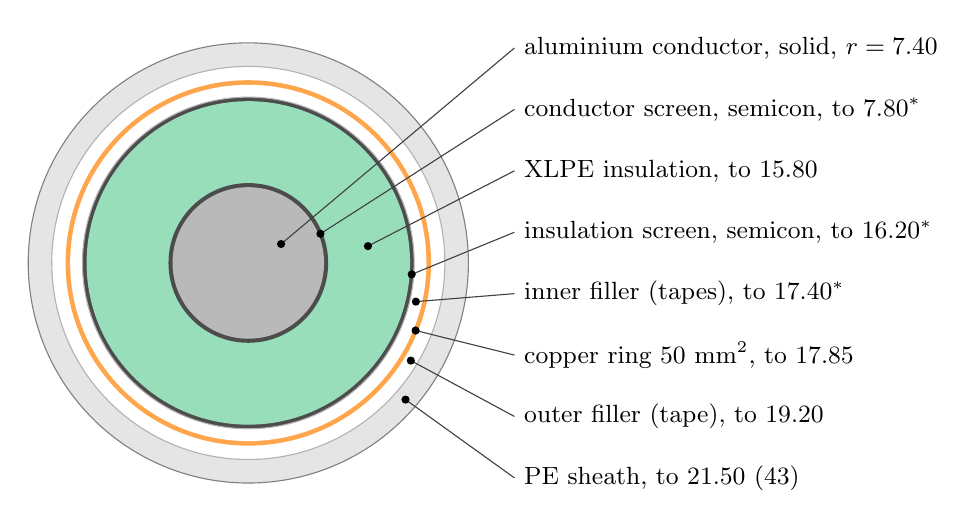
\begin{tikzpicture}[scale=0.13]
\fill[gray!20] (0,0) circle (21.5); \fill[white] (0,0) circle (19.2);
\fill[orange!70] (0,0) circle (17.85); \fill[white] (0,0) circle (17.4);
\fill[black!70] (0,0) circle (16.2); \fill[green!35!teal!40] (0,0) circle (15.8);
\fill[black!70] (0,0) circle (7.8); \fill[gray!55] (0,0) circle (7.4);
\draw[gray] (0,0) circle (21.5); \draw[gray!60] (0,0) circle (19.2); \draw[gray!60] (0,0) circle (16.2);
\foreach \r/\a/\t/\y in {3.7/30/{aluminium conductor, solid, $r=7.40$}/21,
   7.6/22/{conductor screen, semicon, to 7.80$^*$}/15, 11.8/8/{XLPE insulation, to 15.80}/9,
   16.0/-4/{insulation screen, semicon, to 16.20$^*$}/3, 16.8/-13/{inner filler (tapes), to 17.40$^*$}/-3,
   17.625/-22/{copper ring 50 mm$^2$, to 17.85}/-9, 18.52/-31/{outer filler (tape), to 19.20}/-15,
   20.35/-41/{PE sheath, to 21.50 ($\varnothing$43)}/-21}
  {\draw[thin,black!75] (26,\y) node[right,font=\small,black]{\t} -- ({\r*cos(\a)},{\r*sin(\a)});
   \fill[black] ({\r*cos(\a)},{\r*sin(\a)}) circle (0.4);}
\end{tikzpicture}

\figcap{One cable of the model, to scale (radii in mm from its axis; \(^*\) assumed).}\end{center}
The copper wires and tape are one ring of equal area: same DC resistance, no lay. The ring
position only affects the screen loop (Section 3, Q3.4).

\begin{center}% Q1.1: the three cables in trefoil, to scale (mm), same layer colours as cable_section.tex.
% Centre spacing 43.5 mm = 43 mm jacket + 0.5 mm soil gap; origin (+) = trefoil centre.
\begin{tikzpicture}[x=0.7mm, y=0.7mm]
\def\trefS{43.5}\pgfmathsetmacro{\trefH}{sqrt(3)/2*\trefS}
\foreach \x/\y/\p/\ang in {0/{2*\trefH/3}/A/{0^\circ}, {-\trefS/2}/{-\trefH/3}/B/{-120^\circ},
                           {\trefS/2}/{-\trefH/3}/C/{+120^\circ}} {
  \begin{scope}[shift={(\x,\y)}]
    \fill[gray!20] (0,0) circle (21.5); \fill[white] (0,0) circle (19.2);
    \fill[orange!70] (0,0) circle (17.85); \fill[white] (0,0) circle (17.4);
    \fill[black!70] (0,0) circle (16.2); \fill[green!35!teal!40] (0,0) circle (15.8);
    \fill[black!70] (0,0) circle (7.8); \fill[gray!55] (0,0) circle (7.4);
    \draw[gray] (0,0) circle (21.5); \draw[gray!60] (0,0) circle (19.2); \draw[gray!60] (0,0) circle (16.2);
    \node[align=center,inner sep=0pt] at (0,0) {\textbf{\p}\\[-1pt]{\tiny\(\ang\)}};
  \end{scope}}
\draw[thick] (-1.6,0) -- (1.6,0) (0,-1.6) -- (0,1.6);   % trefoil centre = origin
% the 0.5 mm soil gap at the B-C contact: leader straight down through the soil between B and C
\fill[black] (0,{-\trefH/3}) circle (0.5);
\draw[thin,black!75] (0,{-\trefH/3}) -- (0,{-\trefH/3-21});
\node[font=\small,anchor=north,inner sep=1pt] at (0,{-\trefH/3-21}) {0.5 mm gap};
% centre spacing B-C
\draw[thin,gray] ({-\trefS/2},{-\trefH/3-23}) -- ({-\trefS/2},{-\trefH/3-35}) ({\trefS/2},{-\trefH/3-23}) -- ({\trefS/2},{-\trefH/3-35});
\draw[{Latex[length=4pt]}-{Latex[length=4pt]},thin] ({-\trefS/2},{-\trefH/3-32}) -- ({\trefS/2},{-\trefH/3-32})
  node[midway,fill=white,font=\small,inner sep=1.5pt] {43.5 mm};
\end{tikzpicture}

\figcap{The three cables in trefoil, to scale, with the phase angle of each conductor. The jackets are
0.5 mm apart (Q1.2 explains why). The cross marks the trefoil centre, the origin of the model, 1.0 m below
the ground surface.}\end{center}

\begin{table}[H]\centering\small
\caption{Material properties (all are ONELAB parameters in \texttt{parameters.pro}).}
\begin{tabularx}{\linewidth}{@{}l c c c Y@{}}
\toprule Material & \(\varepsilon_r\) & \(\sigma\) at 20\,\(^\circ\)C [S/m] & \(\kappa\) [W/(m K)] & Basis\\\midrule
Aluminium & -- & \(3.544\cdot10^7\), \(\alpha=0.0039\) & 237 & \(\sigma\) fitted to NKT \(R_{DC}\) (61\,\% IACS: \(3.538\cdot10^7\) [NBS], 0.2\,\% apart); \(\alpha\) [Course]; \(\kappa\) [Lee]\\
Copper (screen) & -- & \(5.80\cdot10^7\), \(\alpha=0.00386\) & 402 & annealed Cu, \(\rho=1.7241\cdot10^{-8}\) [NBS]; \(\alpha\) [Course]; \(\kappa\) [Lee]\\
XLPE & 2.5 & \(10^{-18}\) & 0.286 & \(\varepsilon_r\) [\v{S}u\'{c}urovi\'{c}, Lee]; \(\sigma\) [Course, COMSOL]; \(\rho_T=3.5\) K\,m/W [Enescu]\\
Semicons & -- & \(2\cdot10^{-3}\) & 0.286 & \(\sigma\): limit 500 \(\Omega\)m [OES], same value in [Lee]; \(\kappa\) as XLPE (assumption)\\
PE sheath & 2.25 & \(10^{-18}\) & 0.286 & [Course, COMSOL]; \(\rho_T=3.5\) K\,m/W [Enescu]\\
Fillers (tapes) & -- & 0 & 0.286 & assumption: polymer, as XLPE\\
Soil & 10 & \(10^{-2}\) & 0.833 & \(\varepsilon_r,\sigma\) [Course App.~C]; \(\rho_T=1.2\) K\,m/W [NKT]\\
Air (void, Q2.5) & 1 & \(10^{-15}\) & -- & assumption\\
\bottomrule
\end{tabularx}
\end{table}
All materials are non-magnetic (\(\mu_r=1\)): there is no steel. Using 3.5 K\,m/W, the IEC 60287 value for
XLPE and PE [Enescu], for all polymers makes the FE model and the IEC 60287 check of Section 4 use the same data.

\codeguide{\setupfile{parameters.pro}: every value with its basis tag (the sources below,
[DERIVED], [ASSUMPTION]). \setupfile{cable.geo}: the layer radii \texttt{R[]}.}
{Open \setupfile{cable.geo} in Gmsh to see the geometry.}{\texttt{sigmaAl} reproduces 0.164 \(\Omega\)/km by construction.}

\section*{Q1.2 Environment and computational domains}
\assignmentquestion{\QuestionOneTwo}
\answer{\AnsOneTwo}
\textbf{Environment = the NKT rating conditions}: homogeneous soil, thermal resistivity 1.2 K\,m/W
(\(\kappa=0.833\)), 15\,\(^\circ\)C, trefoil centre 1.0 m below the ground surface (we take the depth to
the arrangement centre, as IEC 60287 does for a trefoil group). Air above at 15\,\(^\circ\)C. Soil
electrical data from the course (\(\varepsilon_r=10\), \(\sigma=0.01\) S/m): shielded in the electric model
and negligible in the magnetic one (skin depth \(\approx\)700 m). Soil drying and layering are neglected.

\textbf{Domains (one mesh).} Electromagnetic box \(\pm0.3\) m around the trefoil (Sections 2--3), nested in
a soil rectangle up to the ground surface, \(\pm20\) m wide and 20 m deep (Section 4).

\begin{center}% Q1.2, Q4.2: environment and computational domains (not to scale).
\begin{tikzpicture}[font=\small,>=Stealth]
\fill[KULLight!12] (-7,0) rectangle (7,0.8);
\fill[brown!12] (-7,0) rectangle (7,-3.6);
\draw[KULBlue,very thick] (-7,0) -- (7,0);
\draw[thick] (-7,0) -- (-7,-3.6) -- (7,-3.6) -- (7,0);
\node[anchor=west] at (-6.9,0.4) {air, \(T_{\rm amb}=15\,^\circ\)C};
\node[anchor=east,KULBlue] at (6.9,0.4) {ground surface: \(-\kappa\,\partial_nT=h\,(T-T_{\rm amb})\), \(h=10\) W/(m\(^2\)K)};
\node[rotate=90,anchor=south] at (-7,-1.8) {\(\partial_nT=0\) at \(x=-20\) m};
\node[rotate=-90,anchor=south] at (7,-1.8) {\(\partial_nT=0\) at \(x=+20\) m};
\node[anchor=south] at (0,-3.6) {\(T=T_{\rm amb}=15\,^\circ\)C at 20 m depth};
\node[align=center] at (-3.7,-1.9) {soil: \(\rho_T=1.2\) K\,m/W\\ (\(\kappa=0.833\) W/(m\,K)), 15\,\(^\circ\)C};
\draw[<->] (6.4,0) -- node[pos=0.72,left] {20 m} (6.4,-3.6);
\draw[<->] (-7,-3.0) -- node[above,fill=brown!12,inner sep=1pt] {40 m} (6.4,-3.0);
% EM box with the trefoil
\draw[KULBlue,thick,fill=white] (-0.45,-1.75) rectangle (0.45,-0.85);
\foreach \x/\y in {0/-1.18, -0.13/-1.41, 0.13/-1.41} \fill[black!70] (\x,\y) circle (0.13);
\draw[<->] (-0.75,0) -- node[left] {1.0 m} (-0.75,-1.3);
\draw[dashed,gray] (-0.85,-1.3) -- (-0.45,-1.3);
\draw[KULBlue,->] (0.5,-1.3) -- (1.5,-1.75) node[right,align=left,KULBlue]
  {EM box \(\pm0.3\) m around the trefoil\\ (Sections 2--3; \(a_z=0\) on its edge)};
\end{tikzpicture}

\figcap{Environment and computational domains (not to scale): the electromagnetic box (Sections 2--3) is a
sub-domain of the thermal soil domain (Section 4) in one mesh.}\end{center}
\textbf{Spacing (TA advice).} Exactly touching jackets create zero-angle soil wedges that ruin
the triangles. We leave a 0.5 mm soil gap (centre spacing 43.5 mm instead of 43.0 mm; trefoil figure in Q1.1):
\begin{center}\small
\begin{tabular}{@{}lrr@{}}\toprule
Default mesh & Touching & 0.5 mm gap\\\midrule
Triangles (whole domain) & \MeshTriTouch & \MeshTriGap\\
XLPE triangles, phase A & \MeshXlpeTouch & \MeshXlpeGap\\
Minimum quality \(q=4\sqrt3A/\sum\ell_i^2\) (1 = equilateral) & \MeshQminTouch & \MeshQminGap\\
Triangles with \(q<0.1\) & \MeshBadTouch & \MeshBadGap\\\bottomrule
\end{tabular}
\end{center}
\begin{center}
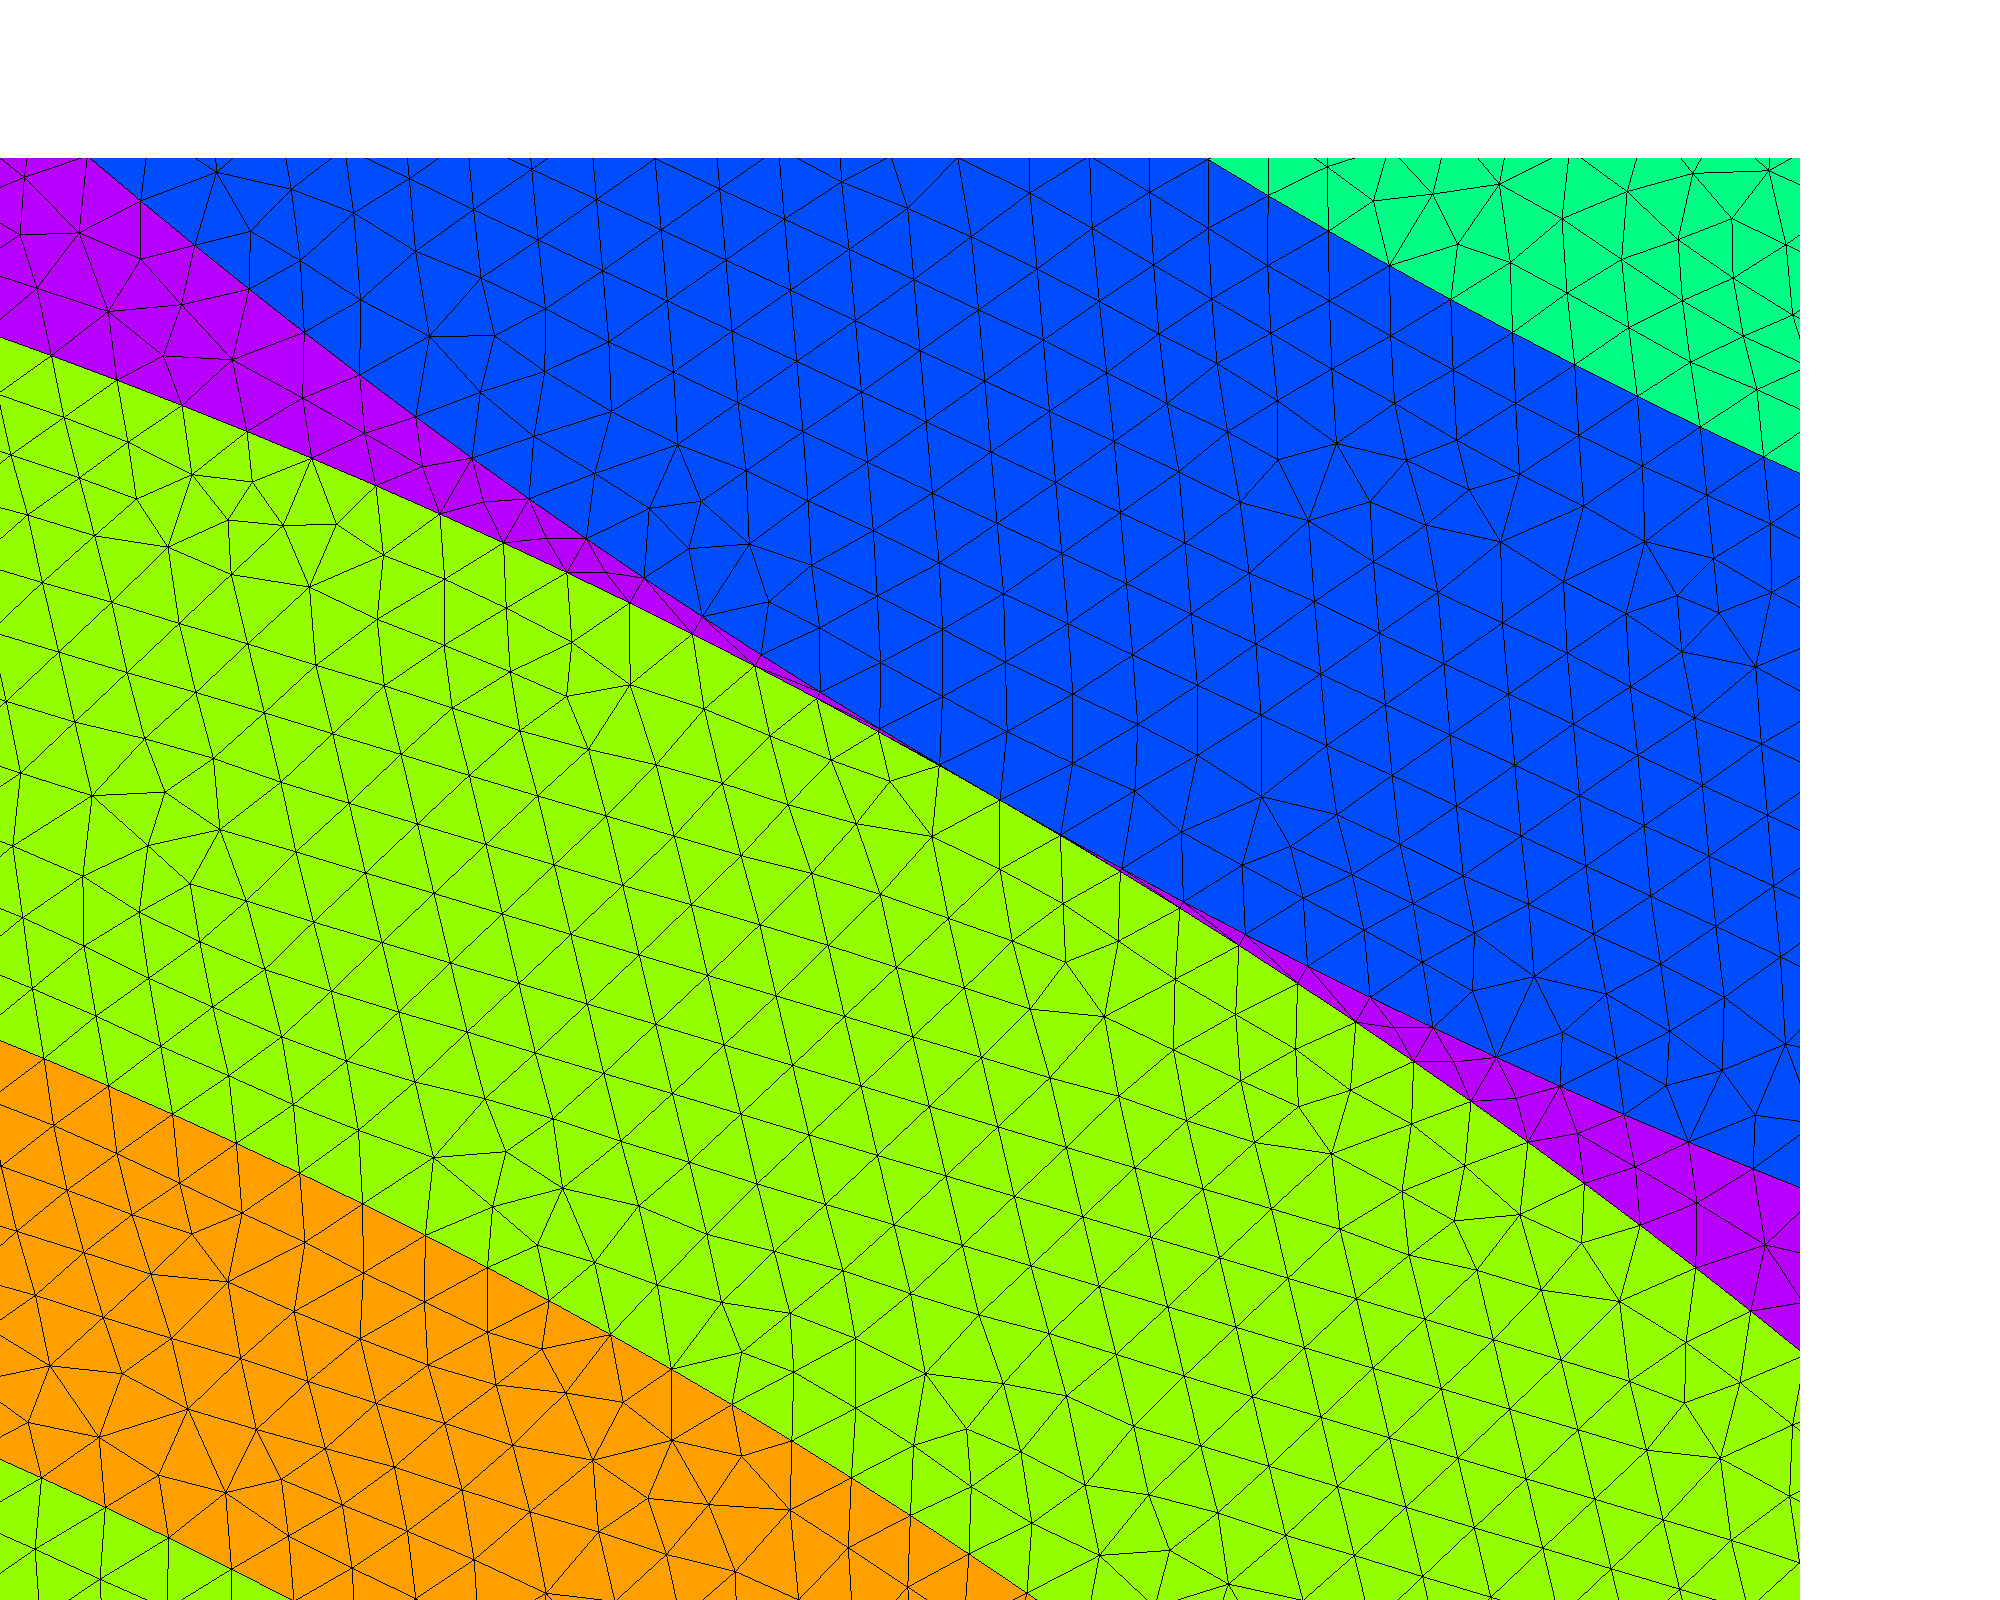
\includegraphics[width=0.4\linewidth,trim=0 70 230 150,clip]{mesh_touching.png}\hspace{4mm}
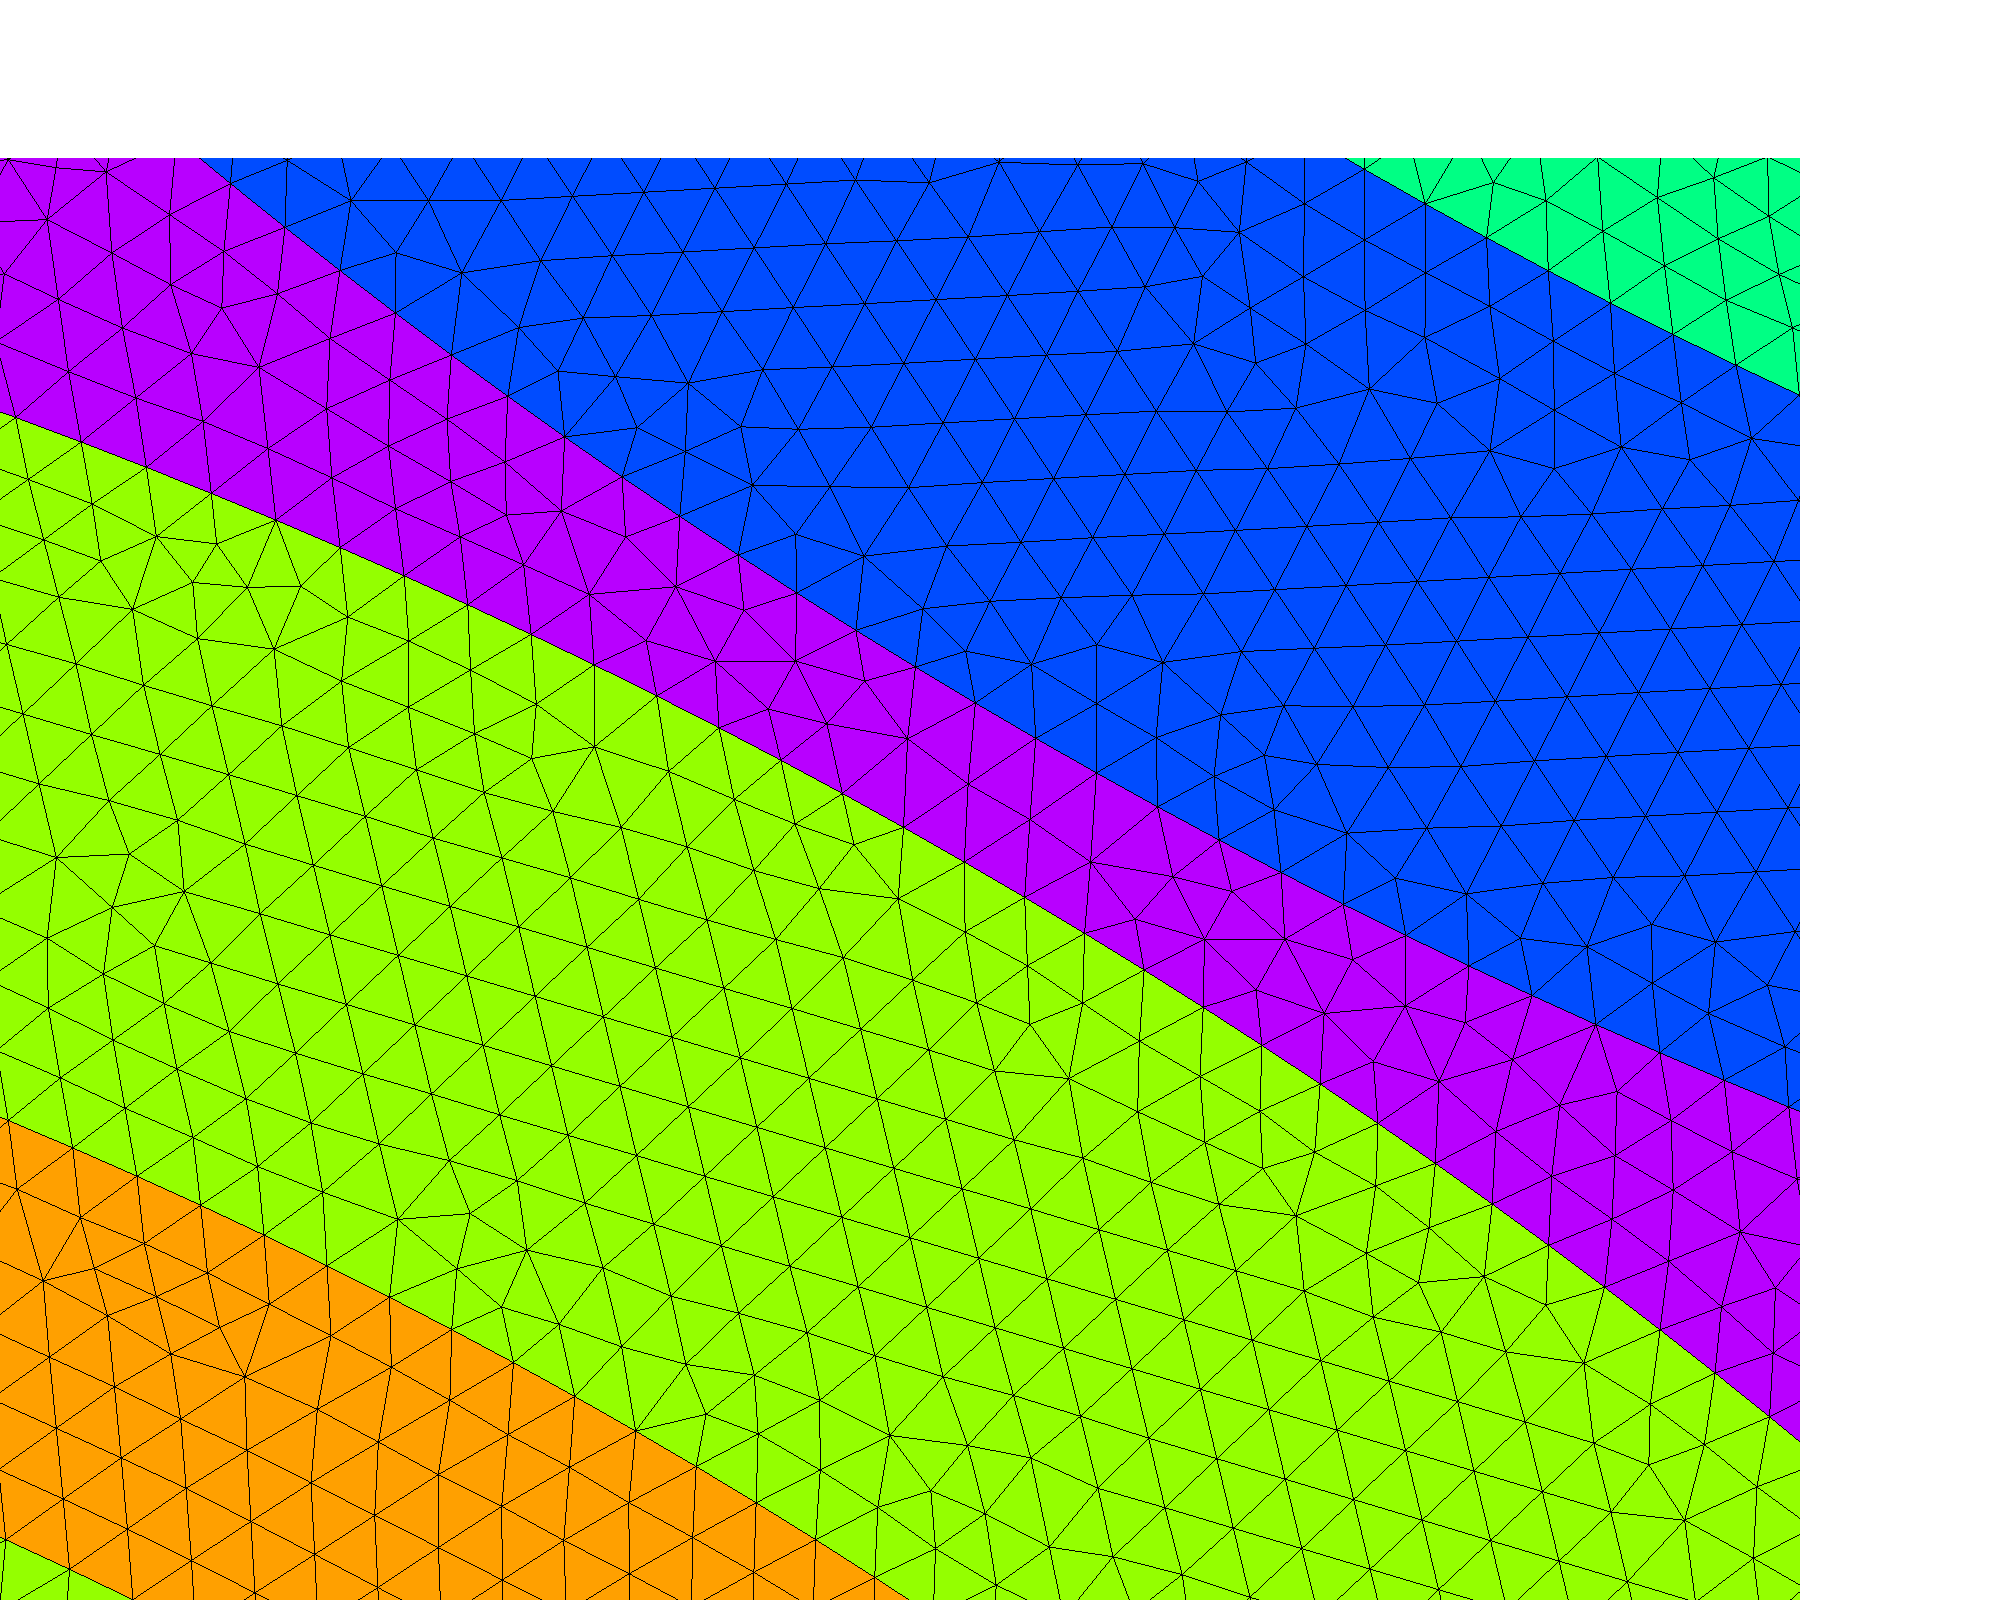
\includegraphics[width=0.4\linewidth,trim=0 70 230 150,clip]{mesh_gap.png}\\
{\small Near a contact point: touching (left) vs 0.5 mm gap (right); colours = layers.}
\end{center}
Sections 2 and 3 quantify the effect of the gap: \(E_{\max}\) \dEtouch\,\%, \(L\) \dLtouch\,\%.

\codeguide{\setupfile{cable.geo}: EM box (group 120), thermal rectangle (98, 130, 132), \texttt{JacketGap}.}
{\runall: meshes \texttt{gap}, \texttt{touching}.}{\texttt{Reports/collect\_values.py} computes the mesh statistics.}

\section*{Q1.3 Sheath bonding}
\assignmentquestion{\QuestionOneThree}
\answer{\AnsOneThree}
\textbf{Both ends bonded} (solid bonding), with ideal earth leads: the bonding of the NKT 350 A
rating row. Circulating screen currents are therefore allowed (Section 3: \(U=0\) per screen).
Single-point bonding (\(I=0\)) is studied as a loss-reduction option (Q3.11, Section 5).
There is no armour or pipe. In the electric model the screens are simply at 0 V.
\begin{center}% Q1.3, Q3.3: screen bonding of the three cables (schematic, one cable section).
\begin{tikzpicture}[font=\small,>=Stealth]
\providecommand{\earth}[1]{\draw (#1) -- ++(0,-0.35); \draw (#1)++(-0.25,-0.35) -- ++(0.5,0);
  \draw (#1)++(-0.16,-0.45) -- ++(0.32,0); \draw (#1)++(-0.07,-0.55) -- ++(0.14,0);}
\foreach \xs/\isopen/\ttl in {0/0/{(a) both ends bonded: \(U_s=0\), \(I_s\neq0\)},
                                    8/1/{(b) single point: \(I_s=0\), \(U_s\neq0\)}} {
  \begin{scope}[xshift=\xs cm]
  \node[anchor=south] at (3,1.95) {\ttl};
  \foreach \y/\p in {1.2/A, 0.7/B, 0.2/C} {
    \draw[orange!80!black,line width=2.2pt] (0.6,\y) -- (5.4,\y);
    \draw[gray!70,line width=0.6pt] (0.4,\y) -- (5.6,\y);
    \node[left] at (0.4,\y) {\p};}
  \draw[thick] (0.6,1.2) -- (0.6,-0.3); \earth{0.6,-0.3}
  \ifnum\isopen=0 \draw[thick] (5.4,1.2) -- (5.4,-0.3); \earth{5.4,-0.3}
    \draw[->,KULBlue,thick] (2.2,1.42) -- node[above,font=\footnotesize] {induced \(I_s\)} (3.8,1.42);
  \else \node[right,font=\footnotesize,align=left] at (5.55,0.45) {open end:\\ standing\\ voltage};
  \fi
  \end{scope}}
\node[font=\footnotesize,gray,anchor=north] at (7,-0.95) {grey: conductor; orange: copper screen; links to earth at the bonded end(s)};
\end{tikzpicture}

\figcap{Both-end bonding (our choice, NKT rating row) closes the screen loop through the earth links, so a
current is induced; single-point bonding leaves one end open, so no net screen current flows.}\end{center}

\section*{Q1.4 Excitation}
\assignmentquestion{\QuestionOneFour}
\answer{\AnsOneFour}
Peak phasors, \(x(t)=\Re\{\hat x\,e^{j\omega t}\}\), 50 Hz, positive sequence A, B, C at
\(0,-120^\circ,+120^\circ\):
\[
 \hat V_k=\frac{\sqrt2\,33}{\sqrt3}e^{-j2\pi k/3}=26.944\,e^{-j2\pi k/3}\ \mathrm{kV},\qquad
 \hat I_k=\sqrt2\,350\,e^{-j2\pi k/3}=494.97\,e^{-j2\pi k/3}\ \mathrm{A}.
\]
\begin{center}% Q1.4: excitation phasors (peak), positive sequence A, B, C.
\definecolor{phB}{HTML}{D1495B}\definecolor{phC}{HTML}{C98A1B}
\begin{tikzpicture}[font=\small,>=Stealth,scale=1.5]
\draw[gray!50,->] (-1.2,0) -- (1.3,0) node[above] {Re}; \draw[gray!50,->] (0,-1.15) -- (0,1.2) node[right] {Im};
\foreach \a/\p/\c/\pos in {0/A/KULBlue/{below right}, -120/B/phB/left, 120/C/phC/left}
  {\draw[->,very thick,\c] (0,0) -- (\a:1) node[\pos,text=\c] {\(\hat V_{\p},\,\hat I_{\p}\)};}
\draw[->,gray] (25:0.45) arc (25:95:0.45) node[pos=0.5,above right] {\(\omega\)};
\node[anchor=west,align=left] at (1.9,0.1) {\(|\hat V_k|=\sqrt2\cdot33/\sqrt3=26.944\) kV\\
  \(|\hat I_k|=\sqrt2\cdot350=494.97\) A\\ angles \(0,\ -120^\circ,\ +120^\circ\); 50 Hz};
\end{tikzpicture}

\figcap{Peak phasors of the three phases at \(t=0\); they rotate counter-clockwise at \(\omega=2\pi\,50\) rad/s.}\end{center}
The voltages drive the electric model, the currents the magnetic one (independent linear problems,
so the load power factor is irrelevant). Results are reported as RMS values and time-averaged losses.

\codeguide{\setupfile{parameters.pro}: \texttt{U\_LL}, \texttt{I\_RMS}, \texttt{Freq}, \texttt{Vpeak}, \texttt{Ipeak}.}
{No solve.}{\(V_p=26944\) V, \(I_p=494.97\) A.}

\subsection*{Sources}
\small
\textbf{[NKT]} \href{../Datasheet NKT 33 kV single core cable XLPE-AL.pdf}{NKT 33 kV single-core XLPE-AL datasheet}, pp.~19--20, 185 mm\textsuperscript2 column.
\textbf{[Course]} \href{../NMES_Assignment_2026.pdf}{NMES assignment 2026}, Appendices A--C.
\textbf{[NBS]} National Bureau of Standards, \refurl{https://nvlpubs.nist.gov/nistpubs/Legacy/hb/nbshandbook100.pdf}{\emph{Copper Wire Tables}, Handbook 100} (1966), \S1.1a, pp.~2--3: annealed copper (IACS) \(\rho=1.7241\cdot10^{-8}\) \(\Omega\)m at 20\,\(^\circ\)C;
\refurl{https://nvlpubs.nist.gov/nistpubs/Legacy/hb/nbshandbook109.pdf}{\emph{Aluminum Wire Tables}, Handbook 109} (1972), Table 1, p.~5: 61\,\% IACS aluminium \(\rho=2.8264\cdot10^{-8}\) \(\Omega\)m.
\textbf{[Lee]} J.-I.~Lee, W.-H.~Jeong, M.-C.~Dinh, I.-K.~Yu, M.~Park, ``Comparative analysis of XLPE and thermoplastic insulation-based HVDC power cables'', \emph{Energies} 16(1), 167 (2023), \S2.3, Table 3 (\(\kappa\): Al 237, Cu 402; semicon \(\sigma=0.002\) S/m; XLPE \(\varepsilon_r=2.5\)), \refurl{https://doi.org/10.3390/en16010167}{doi:10.3390/en16010167} (open access).
\textbf{[\v{S}u\'{c}urovi\'{c}]} M.~\v{S}u\'{c}urovi\'{c} et al., ``FEM-based quantification of eddy-current losses for MV cables in trefoil formation with non-magnetic screens'', \emph{IEEE Access} 14 (2026), Table 1, p.~47244 (19/33 kV cables: XLPE \(\kappa=0.286\), i.e.\ \(\rho_T=3.5\) K\,m/W, \(\varepsilon_r=2.5\), \(\tan\delta=0.004\)), \refurl{https://doi.org/10.1109/ACCESS.2026.3678088}{doi:10.1109/ACCESS.2026.3678088} (open access).
\textbf{[Enescu]} D.~Enescu, P.~Colella, A.~Russo, ``Thermal assessment of power cables and impacts on cable current rating: an overview'', \emph{Energies} 13, 5319 (2020), Table 2, p.~20 (\(\rho_T=3.5\) K\,m/W for XLPE and PE), \refurl{https://doi.org/10.3390/en13205319}{doi:10.3390/en13205319} (open access).
\textbf{[OES]} APSR Oman, \refurl{https://www.dcrp-oman.com/documents/DCRP\%20Updates/OES2\%204th\%20Edition-Circular.pdf}{\emph{OES~2: Cables and Accessories}, 4th ed.} (2024), \S4.1 (33 kV cables), clauses 3 and 5, pp.~20--21: screen volume resistivity \(\le1000\) \(\Omega\)m (conductor screen) and \(\le500\) \(\Omega\)m (insulation screen) at 90\,\(^\circ\)C.
\textbf{[COMSOL]} COMSOL, \refurl{https://doc.comsol.com/6.4/doc/com.comsol.help.models.acdc.submarine_cable_01_introduction/models.acdc.submarine_cable_01_introduction.pdf}{``Submarine Cable 1 -- Introduction''}, Application Gallery documentation (v6.4), materials table, p.~28: XLPE and PE \(\sigma=10^{-18}\) S/m.
\end{document}
